\documentclass[]{article}
\usepackage{packages}
\usepackage{listings}
\usepackage{booktabs}

\newcommand{\ve}[1]{\mathbf{#1}}

\begin{document}

\section{Some shorter questions}
\subsection*{a}
This result can be explained by means of the nuclear shell model. According to this model each sub-level of the nucleus can be identified by 4 quantum numbers $\{n, j, l, m_l\}$. For fixed $\{n, j, l\}$ 
one has that the $2l+1$ sub-levels given by $m_l = -l, -l+1, \dots, l-1, l$ are degenerate and each of these sub-levels can contain two nucleons with different spin z-projrection ($m_s = \pm 1$). \\
At first one can notice that if one sub-shell is filled with two nucleons (of the same type) then the spin contibution of that sub-shell is 0. Having an even number of protons and neutrons means that 
they combine in couples in the sub-shell in a way such that the contribution to the spin of each sub-shell is 0. \\
For what concerns the parity, each particle in the nucleus gives a contribute of $(-1)^l$ due to the orbital motion (the intrinsic parity of the nucleons is $+1$) and the total parity is the product of single parities times the orbital motion contributions. 
The product of the parities of two protons (neutrons) in the same sub-shell is always $+1$ since they, in particular, share the same quantum number $l$. Hence it is legitimate to expect an even-even nucleus
to be in the state $0^+$.
\vspace{10pt} \\
\centerline{\textbf{Answer}: spin $0$, parity $+$}.

\subsection*{b}
The process is governed by the strong interaction, hence quark flavour numbers and baryon numbers must be conserved.
By observing the final state it is immediate to see that the flavour number is 0, and the same holds for the barion number, hence the
hadron must be a meson. \\
By looking at the \href{https://en.wikipedia.org/wiki/Meson#List}{table} of the allowed mesons one can conclude that the isospin $I$ must be either $0$ or $1$. 
On the other side in the final state $I_3=0$ and because of isospin components conservation law one concludes that $I_3=0$ also for the decaying pion.
In conclusion the admitted couples $(I, I_3)$ of isospins are $(0, 0), \ (1, 0)$.

\subsection*{c}
The nuclear potential is charge independent, in the sense that protons and neutrons feel the same nuclear force. It is repulsive for very short distances and attractive for longer dstances (but the force range is short).
In addition a proton feels the effect of the Coulomb interaction with the nucleus, a factor that does not affect the neutron since it is electric neutral. Figure \ref{fig:nucleons_potentials} reports a sketch plot of the 
potentials.
\begin{figure}[hbtp]
    \centering 
    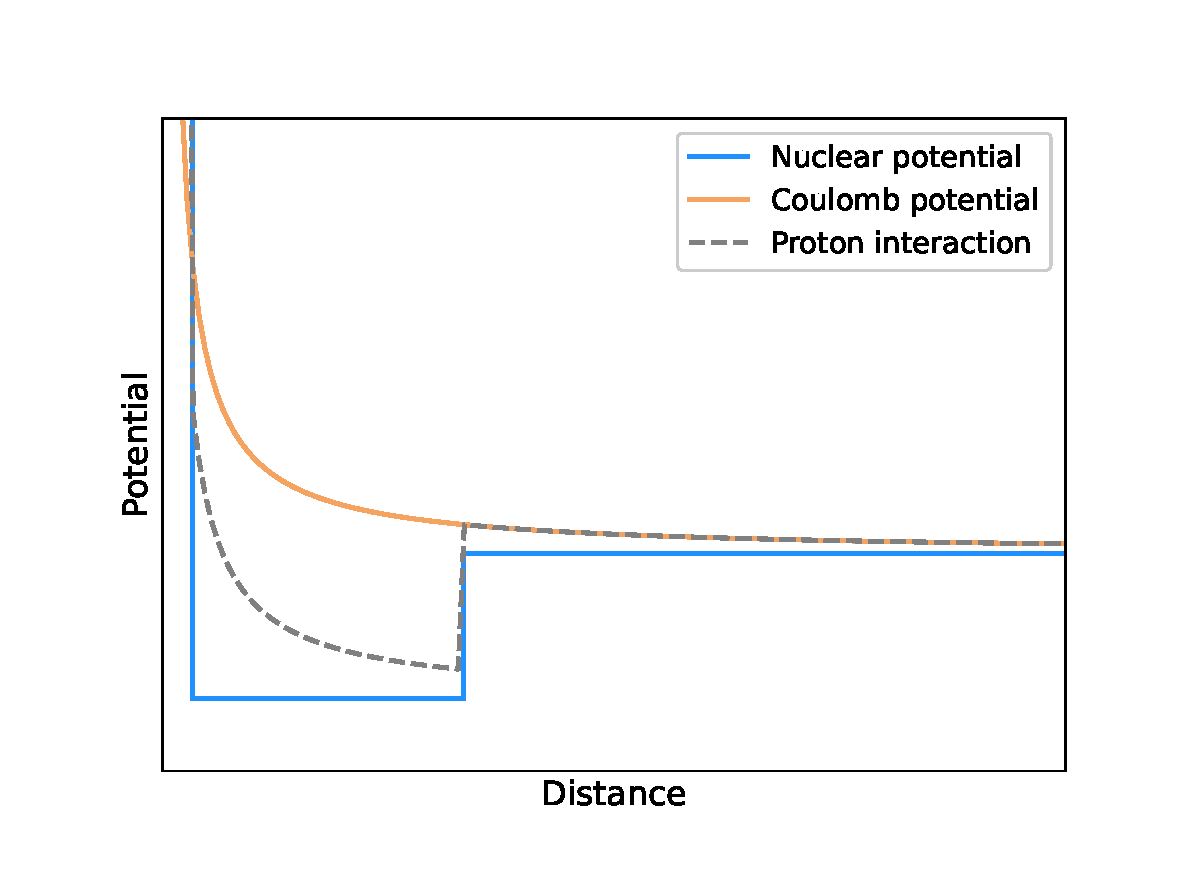
\includegraphics[scale=0.5]{ex1/nucleons.eps}
    \caption{Nucleons interaction. The plot reports  a simplified model of the nuclear potential between two nucleons (blue) and the Coulomb repulsion (orange) which is present
    only for the proton. The grey dotted line represents an approximated potential for the proton, which, in addition, feels also the Coulomb repulsion. The plot is purely qualitative and not in scale.}
    \label{fig:nucleons_potentials}
\end{figure}

\subsection*{d}
The only two other possibilities are the combinations $uuu$ and $ddd$. Since we are dealing with fermions, the \emph{total} wavefunction must be antisymmetric, which means that 
it must be antisymmetric when taking account of all the degrees of freedom. This means that the spatial and spin parts of the wavefunction can be both symmetric or antisymmetric (hence symmetric in total),
provided that the other contributions give an antisymmetric result. Since for $l=0$ the spatial contribution is symmetric, the spin contribution must be itself symmetric. But this is possible only if 
the spins are aligned for a total of $J=3/2$ which contradicts the hypotesis.

\subsection*{e}
The energy to steal a neutron can be calculated by computing the difference between the binding energy $B(A, Z)$ before and after the removal (see exercise 2b for more details). 
\begin{enumerate}
    \item $^{118}Sn \rightarrow B(118, 50) - B(117, 50) \approx 9.03 MeV/c^2$
    \item $^{16}O \rightarrow B(16, 8) - B(15, 8) \approx 15.80 MeV/c^2$
    \item $^{119}Sn \rightarrow B(119, 50) - B(118, 50) \approx 6.54 MeV/c^2$
\end{enumerate}
hence it is harder to steal a neutron from $^{16}O$.

\subsection*{f}
The number of events $N$, the luminosity $\mathcal{L}$ and the cross section $\sigma$ are connected trough the relation
\begin{equation*}
    N = \sigma L
\end{equation*}
and the correct number of events, that is the value that takes account of the efficency $\epsilon$ of the detector and of the backround events number $N_{back}$, is
\begin{equation*}
    N = \frac{N_{obs} - N_{back}}{\epsilon}
\end{equation*}
so that
\begin{equation*}
\sigma= \frac{(N_{obs}-N_{back})}{\epsilon \mathcal{L}} = \frac{984}{0.25 \cdot 5} pb \approx 0.787 pb
\end{equation*} 

\subsection*{g}
Each vertex in the diagram introduces a multiplicative factor of $\alpha = 1/137$ in the probability of the decay to occure, where $\alpha$ is the fine structure constant.
Hence one can expect the probability of a second decay to occur to be approximately $1/137$ of the first one, and the probability of a third decay to be $1/(137)^2$ of the first one. \\
The cross section is a direct measure of the probability of the reaction to occure, hence ratios are expected to be approximately
\begin{equation*}
    1 : \frac{1}{137} : \frac{1}{137^{\, 2}}
\end{equation*}

\section{Nuclear binding energy}
\subsection*{a}
The mass of the atom is given by
\begin{equation*}
    M(^{48}_{20}\text{Ca}^{28}) = Z(m_p + m_e) + (A-Z)m_n - \frac{B(A, Z)}{c^2}
    \label{eq:semi_empirical_mass_formula}
\end{equation*}
where $B$ indicates the binding energy, which in turns can be calculated via the semi-empirical formula (atomic units)
\begin{equation}
    B(A, Z)= a_v A - a_s A^{2/3} - a_c \frac{Z(Z-1)}{A^{1/3}} - a_{sym} \frac{(A - 2Z)^2}{A} + \delta (A, Z)
    \label{eq:semi_empirical_BE_formula}
\end{equation}
where 
\begin{equation*}
    \delta(A, Z) = 
    \begin{cases}
        \frac{a_P}{A^{1/2}} \qquad \text{if Z and N are even} \\
        0 \qquad \text{if A is odd} \\
        -\frac{a_P}{A^{1/2}} \qquad \text{if Z and N are odd} 
    \end{cases}
\end{equation*}
One can simply pop in the values of $A$ and $Z$ into the formula using the fitted coefficients (source Wikipedia) in units of $MeV/c^2$
\begin{equation*}
    a_v = 15.8 \qquad a_s = 18.3 \qquad a_c = 0.714 \qquad a_{sym} = 23.2 \qquad a_P = 12
\end{equation*}
and obtains $B(A, Z) = 412.84~MeV/c^2$. Hence, inserting the result into \ref{eq:semi_empirical_mass_formula} one obtains
\begin{equation*}
    M(^{48}\text{Ca}) \simeq 44670.64~MeV/c^2 \simeq 47.96~u
\end{equation*}
Thhe result is close to the experimental value ($47.952)$. One could justify eventual differences by observing that the SEMF is 
not a complete theoretical model, but rather a fit to experimental data of a model with some theoretical fundations. As such, it is reasonable that the model
can give an overall good description of the data but cannot perfectly describe each of them: this is especially the case of lighter atoms for which
the quantum shell structures of the nucleus should be taken into account.

\subsection*{b}
One can calculate the energy to remove a neutron as the difference in energy between the atom's state wth the neutron and without the neutron. The energy is the sum of
two terms, one that take accounts of the mass of the particles and it is simply the sum of all the masses. The second term, instead, is the binding energy. In the initial and final
state the mass energy contributions are the same (we are not making any particle disappear, we are just moving one away), hence the difference is only due to the binding energy contribution. One can
calculate this contribution as
\begin{equation*}
    B_{neutron} = B(A, Z) - B(A-1, Z)
\end{equation*}
and using expression \ref{eq:semi_empirical_BE_formula} with $A=44$ and $Z=20$ to calculate the two quantities one ends up with an estimation for the energy required to extract the neutron
\begin{equation*}
    B_{neutron} \approx 11.14~MeV/c^2
\end{equation*}

\subsection*{c}
One can search for the most stable atom with fixed $A$ searching for the minimum of the mass formula
\begin{equation*}
    M_A(Z) = Z(m_p + m_e) + (A-Z)m_n - B_A(Z)
\end{equation*}
Since one does not know if $Z$ is even or odd in advance, one can set the pairing term in the binding energy to $0$: this will lead to a non-integer $Z$ and 
the true minimum value will be either the closest greater or smaller integer (one has to check which of the two has minimum energy).
By direct calculation
\begin{equation*}
    0 = \frac{dM_A}{dZ} = m_p + m_e - m_n - \frac{a_c}{A^{1/3}} \left(A-2Z\right) + 4\frac{a_{symm}}{A} \left(A-2Z\right)
\end{equation*}
and rearranging terms
\begin{equation*}
    Z = \frac{m_n - (m_p + m_e) + 4a_{symm}A + a_c A^{2/3}}{2a_c A^{2/3} + 8a_{symm}} \approx 56.59 \qquad \longrightarrow \qquad Z = 56
\end{equation*}

\begin{figure}[h]
    \centering
    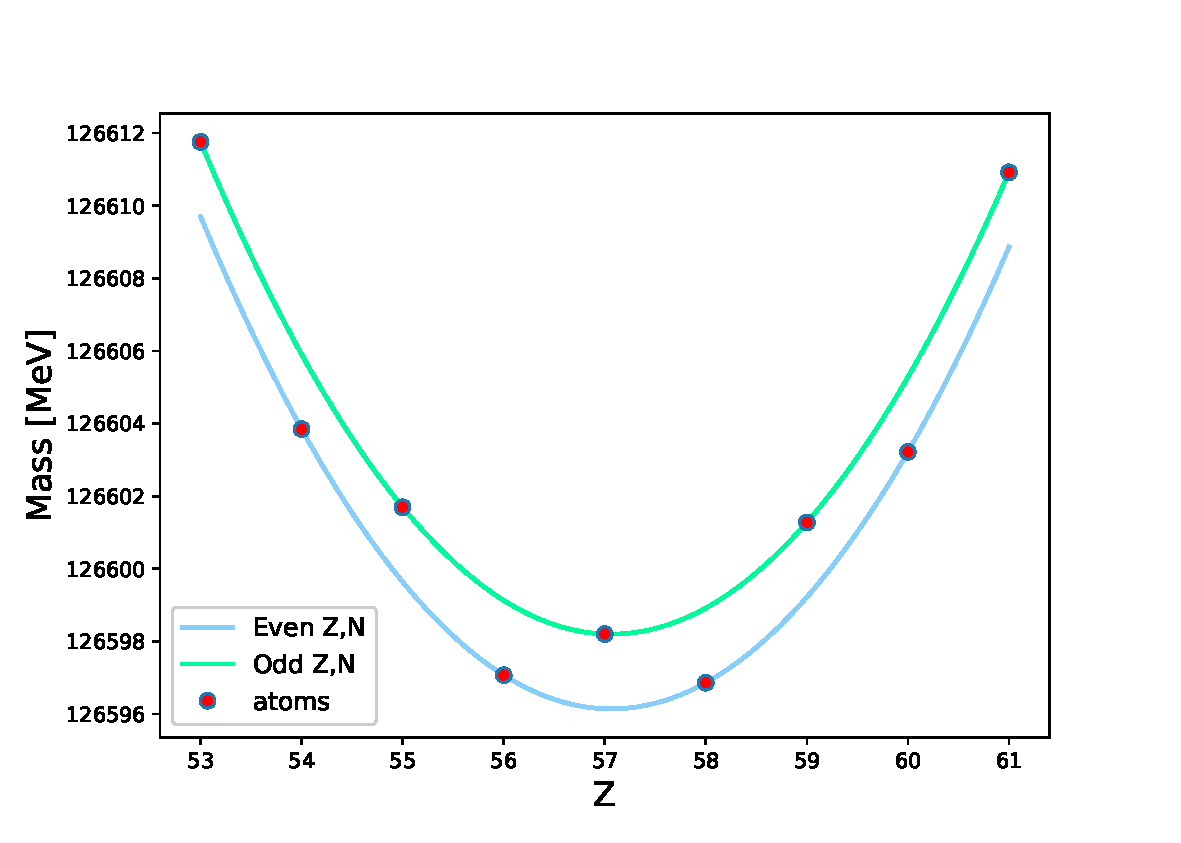
\includegraphics[scale=0.5]{ex2/evenA.eps}
    \caption{Even A}
\end{figure}
\begin{figure}[h]
    \centering
    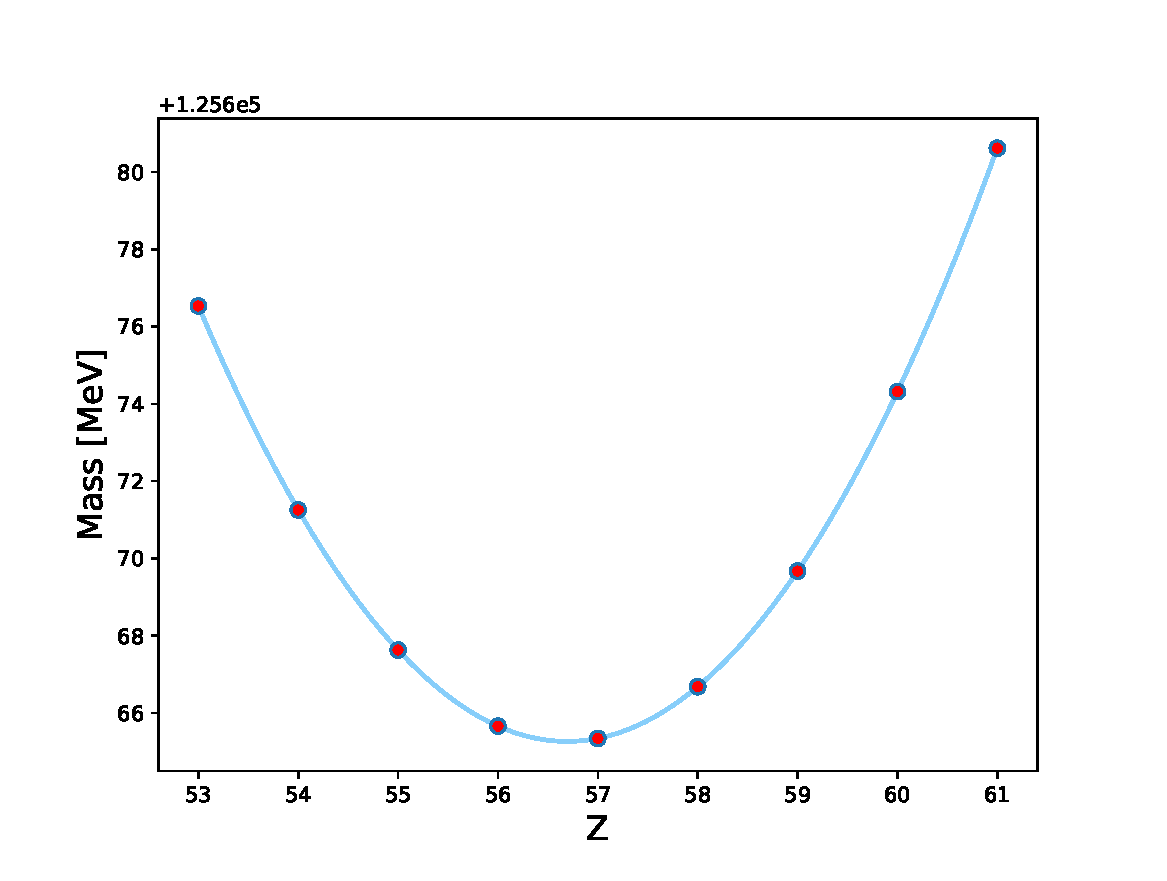
\includegraphics[scale=0.5]{ex2/oddA.eps}
    \caption{Odd A}
\end{figure}

\section{Higgs boson decay}
\subsection*{a}
In the resting frame of the Higgs boson the invariant mass is (atomic units)
\begin{equation}
    W = \sqrt{(\sum_i E_i)^2 - |\sum \ve{p}_i|^2} = E_H = m_H
    \label{eq:W_Higgs_frame}
\end{equation}
The invariant mass is a Lorent invariant, hence this quantity is the same that one observer would measure in the laboratory frame. 
More specifically, one can calculate $W$ after the process using the electrons data
\begin{equation*}
    W = \sqrt{(\sum_i E_i)^2 - |\sum \ve{p}_i|^2} = \sqrt{(\sum_i E_i)^2} = \sqrt{\sum \sqrt{m_i^2 + p_i^2}}
\end{equation*}
By equating this expression to \ref{eq:W_Higgs_frame} and inserting the given values together with the electrons mass one obtains
\begin{equation*}
    m_h \simeq 
\end{equation*}

\subsubsection*{b}
In principle each pair of electron-positron can be generated by the $Z$ boson, in the sense that no rules would be violated. 
In other words there are $4$ different ways to combine the couples of electron-positron to the bosons
\begin{enumerate}
    \item $Z \rightarrow e^+_1 + e^-_1, \quad Z^* \rightarrow e^+_2 + e^-_2$
    \item $Z \rightarrow e^+_1 + e^-_2, \quad Z^* \rightarrow e^+_2 + e^-_1$ 
    \item $Z \rightarrow e^+_2 + e^-_1, \quad Z^* \rightarrow e^+_1 + e^-_2$
    \item $Z \rightarrow e^+_2 + e^-_2, \quad Z^* \rightarrow e^+_1 + e^-_1$
\end{enumerate}
One can now impose the conservation of the $4-$momentum in the bosons' decay and in particular, for the $Z$ boson, this means 
\begin{gather*}
    E_Z = \sqrt{m_Z^2 + p_Z^2} = E_{e^+} + E_{e^-} = \sqrt{m_{e^+}^2 + p_{e^+}^2} + \sqrt{m_{e^-}^2 + p_{e^-}^2} \\
\end{gather*}
and by rearrangin terms
\begin{gather*}
    p_Z^2 = (E_{e^+} + E_{e^-})^2 - m_Z^2
\end{gather*}
this equation gives the value of the momentum that the $Z$ boson must have in order to satisfy the conservation of the energy.
By explicit calculation for the $4$ cases one obtains 
\begin{enumerate}
    \item $p_Z^2 \simeq -2414~GeV/c$
    \item $p_Z^2 \simeq -7350~GeV/c$
    \item $p_Z^2 \simeq 744~GeV/c$
    \item $p_Z^2 \simeq  -5872~GeV/c$
\end{enumerate}
hence only in the third case the particle can be regarded as physical and not virtual.

\subsection*{c}
\subsection*{d}

\section{Lepton universality}
\subsection*{a}
Let us consider the two decays 
\begin{gather*}
    \tau^- \rightarrow \mu^- \, \bar\nu_{\mu} \, \nu_{\tau} \\
    \mu^- \rightarrow e^- \, \bar\nu_e \, \nu_{\mu}
\end{gather*}
represented by the two Feynman diagrams \\
\begin{figure}[hbtp]
    \centering
    \begin{minipage}{0.4\textwidth}
        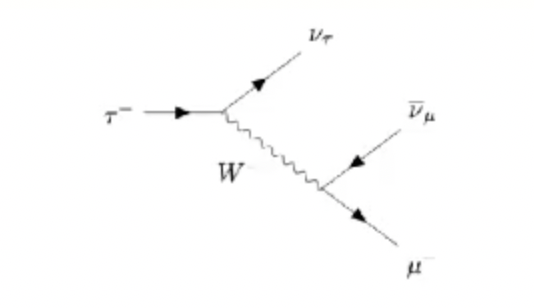
\includegraphics[scale=0.6]{ex4/tau.png}
        \caption{Feynman diagram for the reaction $\tau^- \rightarrow \mu^- \, \bar\nu_{\mu} \, \nu_{\tau}$}
    \end{minipage}
    \hfill
    \begin{minipage}{0.4\textwidth}
        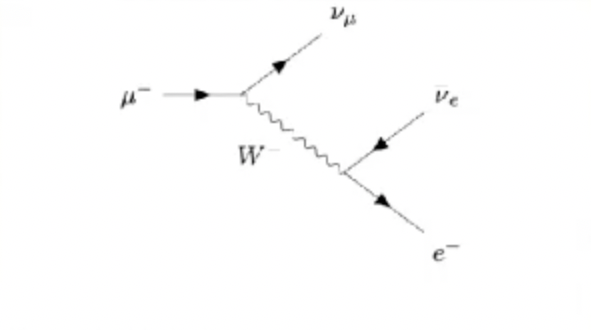
\includegraphics[scale=0.6]{ex4/mu.png}
        \caption{Feynman diagram for the reaction $\mu^- \rightarrow e^- \, \bar\nu_e \, \nu_{\mu}$}
    \end{minipage}
\end{figure}
The probability for a particle to get scattered by a certain potential is proportional to the squared of the so called \emph{amplitude} $\mathcal{M}$.
Assuming that the coupling constant $g^2$ of the Yukawa potential (atomic units)
\begin{equation*}
    V(r) = -\frac{g^2}{4\pi} \frac{e^{-r/R}}{r}
\end{equation*}
is small compared to $4\pi$ (this means that the potential can be considered as a perturbation to the free particle solution), then the amplitude $\mathcal{M}$ of the proces can be computed by means of the Born approximation
\begin{equation*}
    \mathcal{M}(\ve p) = \int V(\ve{r}) \, \exp(i\ve{r}\cdot\ve{r}) \, d^3\ve{r}
\end{equation*}
where $\ve{p} = \ve{p}_i - \ve{p}_f$ denotes the momentum difference between the initial and final state. By direct computation one can prove that 
\begin{equation}
    \mathcal{M}(\ve p) = \mathcal{M}(p^2) = - \frac{g^2}{p^2 + m_x^2}
    \label{eq:amplitude_born}
\end{equation}
where $m_x$ denotes the mass of the propagator. A multiplicative factor of $\sqrt{2}$ must be added if the spin interaction is taken into account. \\
In addition, the force carrier that governs the interaction is the $W$ boson, the mass of which is many times bigger than all the other involved masses. Hence a more suitable form of 
\ref{eq:amplitude_born} is 
\begin{equation*}
    \mathcal{M}(\ve p) = \mathcal{M}(p^2) = - \sqrt{2} \, \frac{g^2}{m_x^2} \approx 1.166 \cdot 10^{-5}~(GeV)^{-2} \equiv G_F
\end{equation*}
and $G_F$ is the Fermi coupling constant.
This results is known as \emph{leptons universality} and states that the amplitude of a lepton's decay process is a constant that does not depend on the chosen lepton. \\
At this point one can introduce the decay rate $\Gamma$ which is proportional to the probability of the process to occur
\begin{equation*}
    \Gamma \approx K M^2 A
\end{equation*}
where $A$ is a constant whose units are those of an energy to the fifth power, because $[M^2] = (GeV)^{-4}$. Since we expect the decay rate 
to depend on the generating particle, a reasonable choice for $A$ is $A=m_i^5$ where indeed $m_i$ denotes the mass of the generating particle. Hence
\begin{equation*}
    \Gamma \approx - \sqrt{2} K \, \frac{g^2}{m_x^2}m_i^5
\end{equation*}
Applying it to the particular case of the two given processes one obtains
\begin{equation}
    \frac{\Gamma\left(\tau^- \rightarrow \mu^- \, \bar\nu_{\mu} \, \nu_{\tau}\right)}{\Gamma\left( \mu^- \rightarrow e^- \, \bar\nu_e \, \nu_{\mu}\right)}
    \approx \left(\frac{m_{\tau}}{m_{\mu}}\right)^5 \approx 1.34 \cdot 10^6
    \label{eq:decay_widths_ratios}
\end{equation}

\subsection*{b}
The two relevant experimental quantities are the lifetime of the particles $\tau$ and the brancing ratios of the reactions. Let us define
$\Gamma_{\tau} \equiv \Gamma(\tau \to X \nu_{\tau})$ and $\Gamma_{\mu} \equiv \Gamma(\tau \to Y \nu_{\mu})$. Equation \ref{eq:decay_widths_ratios} 
can be rewritten as 
\begin{equation*}
    \frac{\Gamma\left(\tau^- \rightarrow \mu^- \, \bar\nu_{\mu} \, \nu_{\tau}\right)}{\Gamma\left( \mu^- \rightarrow e^- \, \bar\nu_e \, \nu_{\mu}\right)} =
    \frac{\Gamma\left(\tau^- \rightarrow \mu^- \, \bar\nu_{\mu} \, \nu_{\tau}\right)}{\Gamma_{\tau}} \
    \frac{\Gamma_\mu}{\Gamma\left( \mu^- \rightarrow e^- \, \bar\nu_e \, \nu_{\mu}\right)} \
    \frac{\Gamma_{\tau}}{\Gamma_{\mu}} = 
    \frac{B\left(\tau^- \rightarrow \mu^- \, \bar\nu_{\mu} \, \nu_{\tau}\right)}{B\left( \mu^- \rightarrow e^- \, \bar\nu_e \, \nu_{\mu}\right)} \ 
    \frac{\tau_{\mu}}{\tau_{\tau}}
\end{equation*}
which is a more relevant form for the experimental quantities.

\section{Quantum numbers}
\subsection*{a} 

\vspace{10pt}
\emph{Parity} \\
\vspace{10pt} \\
Let us consider a wavefunction $\psi(\ve r)$. One can define the parity operator $\hat P$ as an operator such that 
\begin{equation*}
    \hat P \, \psi(\ve r) = \psi(-\ve r)
\end{equation*}
Since
\begin{equation}
    \hat P^2 \, \psi(\ve r) = \hat P \, \psi(-\ve r) = \psi(\ve r)
    \label{eq:eigenvalue_equation_parity}
\end{equation}
the eigenvalues of the parity operator are $\pm 1$ and the corresponding eigenfunctions are the odd (eigenvalue $-1$) and even (eigenvalue $+1$) wavefunctions. If the wavefunction
describes the state of particle, and the state is an eigenstate of the parity operator, the corresponding eigenvalue is also said to be the (intrinsic) parity of the particle. Formally
\begin{equation*}
    \hat P \psi(\ve r) = \pi \psi(\ve r)
\end{equation*}
and $\pi$ is the (intrinsic) parity of the particle. \\
Let us consider a system of two particles $A+B$ described by a wavefunction $\psi_{AB}(\ve{r}_A, \ve{r}_B)$. It can be proven that the parity of the system is given by 
\begin{equation*}
    \hat P \psi_{AB} = \pi_A \pi_B (-1)^l \psi_{AB}
\end{equation*}
where $l$ denotes the orbital angular momentum quantum number of the relative motion. Hence in a reaction of the type $A+B \rightarrow C+D$ described by a hamiltonian $\hat H$ that commutes with parity,
parity is conserved or, in other words
\begin{equation*}
    \pi_A \pi_B (-1)^{l_{AB}} = \pi_C \pi_D (-1)^{l_{CD}} 
\end{equation*}
This, for example, is not the case of the weak interaction where, in general, the hamiltonian operator does not commute with the parity operator. \\
\vspace{10pt} \\

\raggedright\emph{Charge conjugation} \\
\vspace{10pt} 
The charge conjugation operator is an operator that changes the sign of all the forces' quantum charges, specifically electric charge, baryon number, lepton number, flavor charges, isospin, \dots In particular, if applied to a particle, the C-parity operator 
transforms the particle into its antiparticle. If a particle is in a state $\left| \psi \right\rangle$ then the action of the conjugation operator reads 
\begin{equation*}
    \hat C \, \left| \psi \right\rangle = \left| \bar\psi \right\rangle
\end{equation*}
where $\left| \bar\psi \right\rangle$ represents the antiparticle's state. \\
The eigenstates of the C-parity operator are the systems neutral to all force charges like the photon or particle-antparticle bound states. In this case
\begin{equation*}
    \hat C \, \left| \psi \right\rangle = C_{\psi} \left| \psi \right\rangle
\end{equation*}
and $C_{\psi}$ is said to be the C-parity of the particle. As for the the parity operator, the eigenvalues can be only $\pm 1$. \\
Both P-parity and C-parity are conserved in the processes governed by all the fundamental forces \href{https://en.wikipedia.org/wiki/Weak_interaction#Violation_of_symmetry}{but the weak force}.

\subsection*{b}
The notation $^3S_1$ stands for $L=1$ $S=1$ and $J=1$. The $J/\Psi$ Meson is a bound state of a charm quark and an anti-charm quark. By applying the C-parity operator on the state $\left|J/\Psi\right\rangle$ and noting that each quark simply swap their roles,
one obtains that the C-parity of the $J/\psi$ meson is -1 (the only contribution is due to the angular momentum).
\begin{equation*}
    \hat C \left|J/\Psi\right\rangle = (-1)^J\left|J/\Psi\right\rangle = -\left|J/\Psi\right\rangle
\end{equation*}
\subsection*{c}
$^{15}$N atom has 7 protons and 8 neutrons. Since the neutrons (in the ground state) are all coupled (each sub-shell admits two nucleons) they do not contribute to  the spin of the nucleus and the parity contribution is $+1$. Instead the protons configuration
of the $^{15}$N atom in the ground state is $(1s)^2 \, (1p_{3/2})^4 \, (1p_{1/2})^1$: only the last proton contributes to the interested quantities. Since the orbital $p$ represents the quantum number $l=1$ the parity of the the nucleus is the product of the neutrons 
an protons contribution, that is $(+1) \cdot (-1)^1 = -1$. The spin is then $1/2$. \\ \newpage
There are three possible alternatives for the first excited state, all of which consist in moving a proton or a neutron to another level starting from the ground state configuration.
\begin{enumerate}
    \item Move the $1p_{1/2}$ proton to the $1d_{5/2}$ level (figure \ref{fig:nitrogen_nucleons_excited_states} on the left) \\ $\quad \longrightarrow \quad$ the new proton configuration is $(1s)^2 \, (1p_{3/2})^4  \, (1d_{5/2})^1$ and the spin-parity is $5/2^+$.
    \item Move the $1p_{1/2}$ neutron to the $1d_{5/2}$ level (figure \ref{fig:nitrogen_nucleons_excited_states} in the middle) \\ $\quad \longrightarrow \quad $ the new neutron configuration is $(1s)^2 \, (1p_{3/2})^4 \, (1p_{1/2})^{1} \, (1d_{5/2})^1$. The parity here is non-trivial because of the angular momemnta addition rules.
    \item Move the $1p_{3/2}$ proton to the $1p_{1/2}$ level (figure \ref{fig:nitrogen_nucleons_excited_states} on the right)\\ $\quad \longrightarrow \quad$ the new proton configuration is $(1s)^2 \, (1p_{3/2})^{3} \, (1p_{1/2})^2$ and the spin-parity is $3/2^-$.
\end{enumerate}
By looking at the suggested table, one can notice that the first excited state is described by configuration $1$, the second excited state by configuration $2$ and the third excited state is described by configuration $3$.


\begin{figure}
    \centering
    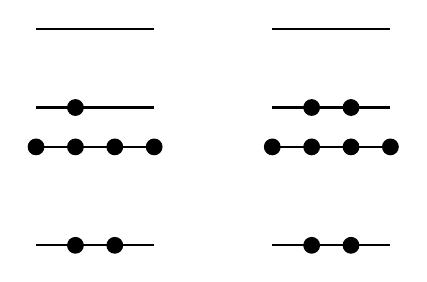
\begin{tikzpicture}
        
        % Protons
        \foreach \x in {0, 3}{
            \foreach \y in {0, 1.25, 1.75, 2.75}{
                \draw [thick] (\x, \y) -- ++(1.5, 0);
            }
            \node[draw, circle, inner sep=2pt, fill] at (\x+0.5, 0){};
            \node[draw, circle, inner sep=2pt, fill] at (\x+1, 0)(1.5,0){};
            \node[draw, circle, inner sep=2pt, fill] at (\x, 1.25){};
            \node[draw, circle, inner sep=2pt, fill] at (\x+0.5, 1.25){};
            \node[draw, circle, inner sep=2pt, fill] at (\x+1.5, 1.25){};
            \node[draw, circle, inner sep=2pt, fill] at (\x+1, 1.25){};
            \node[draw, circle, inner sep=2pt, fill] at (\x+0.5, 1.75){};
        }
        \node[draw, circle, inner sep=2pt, fill] at (4, 1.75){};
    \end{tikzpicture}
    \caption{Ground state $^{15}$N nucleus configuration}
    \label{fig:nitrogen_nucleons_ground_state}
\end{figure}


\begin{figure}
    \centering
    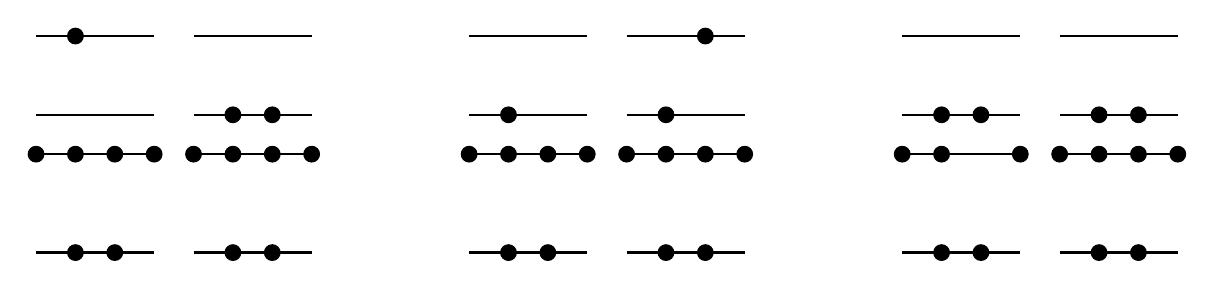
\begin{tikzpicture}

        % Protons
        \foreach \x in {0.5, 6, 11.5}{
            \foreach \y in {0, 1.25, 1.75, 2.75}{
                \draw [thick] (\x, \y) -- ++(1.5, 0);
            }
            \node[draw, circle, inner sep=2pt, fill] at (\x+0.5, 0){};
            \node[draw, circle, inner sep=2pt, fill] at (\x+1, 0)(1.5,0){};
            \node[draw, circle, inner sep=2pt, fill] at (\x, 1.25){};
            \node[draw, circle, inner sep=2pt, fill] at (\x+0.5, 1.25){};
            \node[draw, circle, inner sep=2pt, fill] at (\x+1.5, 1.25){};
        }
        
        % 1p 1/2 proton
        \node[draw, circle, inner sep=2pt, fill] at (1, 2.75){};
        \node[draw, circle, inner sep=2pt, fill] at (6.5, 1.75){};
        \node[draw, circle, inner sep=2pt, fill] at (12, 1.75){};

        % 1p 1/2 neutron
        \node[draw, circle, inner sep=2pt, fill] at (3.5, 1.75){};
        \node[draw, circle, inner sep=2pt, fill] at (9, 2.75){};
        \node[draw, circle, inner sep=2pt, fill] at (14.5, 1.75){};

        % 1p 3/2 proton
        \node[draw, circle, inner sep=2pt, fill] at (1.5, 1.25){};
        \node[draw, circle, inner sep=2pt, fill] at (7, 1.25){};
        \node[draw, circle, inner sep=2pt, fill] at (12.5, 1.75){};

        % Neutrons
        \foreach \x in {2.5, 8, 13.5}{
            \foreach \y in {0, 1.25, 1.75, 2.75}{
                \draw [thick] (\x, \y) -- ++(1.5, 0);
            }
            \node[draw, circle, inner sep=2pt, fill] at (\x+0.5, 0){};
            \node[draw, circle, inner sep=2pt, fill] at (\x+1, 0)(1.5,0){};
            \node[draw, circle, inner sep=2pt, fill] at (\x, 1.25){};
            \node[draw, circle, inner sep=2pt, fill] at (\x+0.5, 1.25){};
            \node[draw, circle, inner sep=2pt, fill] at (\x+1, 1.25){};
            \node[draw, circle, inner sep=2pt, fill] at (\x+1.5, 1.25){};
            \node[draw, circle, inner sep=2pt, fill] at (\x+0.5, 1.75){};
        }

    \end{tikzpicture}
    \caption{First three excited states of a $^{15}$N nucleus}
    \label{fig:nitrogen_nucleons_excited_states}
\end{figure}

\subsection*{d}
The third excited state is the one that has $J^p = \frac{3}{2}^-$. From this state the nucleus can decay into the second excited state, the first excited state and the ground state. 
Let us first consider the decay to the ground state. When the excited proton returns to the $1p_{3/2}$ level there is no change in parity 
and one has that $\Delta J = J_{exc} - J_{ground} = 1$. This means that one must have odd-L magnetic fields and even-L electric fields. \\
Because of the general selection rules in the gamma decays one has that, said $L$ the photon's angular momentum
\begin{gather*}
    |J_{exc} - J_{ground}| \leq L \leq J_{exc} + J_{ground} \qquad \longrightarrow \qquad 1 \leq L \leq 2
\end{gather*}
The allowed states are
\begin{equation*}
    M_1, E_2
\end{equation*}
For $A=15$ one has that (reference chapter 10.3 Krane)
\begin{equation}
    \frac{\lambda(E_2)}{\lambda(M_1)} \approx 10^{-3}
\end{equation}
hence we expect the $M_1$ decay to be the most probable one, but with a non-neglectable contribution of $E_2$. \\
In an analogous way one can find that for the decays to the second and first excited states the relations reported in table \ref{tab:gamma_transitions}.
\begin{table}[htbp]
    \centering
    \begin{tabular}{cccccc}
        \toprule
        Transition & $\Delta E$ & $\Delta \pi$ & $L$ & Fields & Dominants\\
        \midrule
        $3 \to 0$ & $\approx 6.3~MeV$ & no & $1 \leq L \leq 2$ & $M_1, E_2$ & $M_1, E_2$ \\
        $3 \to 1$ & $\approx 1~MeV$ & yes & $1 \leq L \leq 4$ & $E_1, M_2, E_3, M_4$ & $E_1$\\
        $3 \to 2$ & $\approx 1~MeV$ & yes & $1 \leq L \leq 2$ & $E_1, M_2$ & $E_1$ \\
        \bottomrule
    \end{tabular}
    \caption{$\gamma$ transitions from the $3$rd excited state}
    \label{tab:gamma_transitions}
\end{table}
For the transition $2 \to 1$ one has that the dominant field is $E_2$ ($2 \leq L \leq 3$ and no parity change) while for the decay 
$2 \to 0$ the dominant field is $E_1$ ($0 \leq L \leq 1$ and parity change). Hence from the second excited state the nucleus can decay to the ground state 
via $E_1$ radiation, or it can decay to the first excited state via $E_2$ radiation. By comparing probabilities (reference chapter 10.3 Krane)
\begin{equation*}
    \frac{P_{2 \to 0}}{P_{2 \to 1}} \approx \frac{\lambda(E_1)}{\lambda(E_2)} = \frac{1}{7.3} \cdot 10^{7} \cdot  A^{-2/3} > 1
\end{equation*}

\section{Allowed, suppressed and forbidden processes}
I use the definition of decay stated \href{https://en.wikipedia.org/wiki/Particle_decay}{here}
\subsection*{a}
\begin{table}[htbp]
    \centering
    \begin{tabular}{cccccc}
        \toprule
            Process & Type & Interaction & Allowed & Suppressed & Reason not allowed \\
        \midrule 
            $1$ & decay & electroweak & yes & no & \\
            $2$ & & & no & & charge \\
            $3$ & decay & electroweak & yes & yes & \\
            $4$ & decay & weak & yes & yes & \\
            $5$ & decay & strong & yes & yes & \\
            $6$ & reaction & electroweak + strong & yes & yes & \\
            $7$ & decay & weak & yes & yes & \\
            $8$ & & & no & & lepton number \\
        \bottomrule
    \end{tabular}
\end{table}
\subsection*{b}
\subsection*{c}
\begin{itemize}
    \item Let us consider the decay 1. One can estimate the average lifetime $\tau$ of $\psi(3086)$ as the squared inverse of the coupling constant, hence
    \begin{equation*}
        \tau \approx 
    \end{equation*}
    The experimental known lifetime is \footnote{}. \\
    \item For the decay $3$ the lifetime can be estimated as $\tau \approx \frac{1}{G_F^2} \approx 10^{-12}$ which is compatible with the \href{http://hyperphysics.phy-astr.gsu.edu/hbase/Particles/qrkdec.html}{experimental value}
    \item For the decay $7$ the lifetime can be estimated as 
\end{itemize}
\subsection*{d}
\subsection*{e}

\section{Radioactive decay}
\subsection*{a}
Said $N(t)$ the number of atoms present at time $t$, the radioactive decay law states that
\begin{equation}
    \mathcal{A} = -\frac{dN}{dt} = \lambda N
    \label{eq:decay_law}
\end{equation}
where $\lambda$ is called the decay constant. \\
By integrating it in time one obtains 
\begin{equation}
    N(t) = N_0 \, e^{-\lambda t}
    \label{eq:decay_chain_first_atom}
\end{equation}
Now if we consider a chain decay of the type $A \rightarrow B \rightarrow C$ with initial conditions 
\begin{equation*}
    N_A(t=0) = N_0 \qquad N_B(t=0) = N_C(t=0) = 0
\end{equation*}
one can immediately obtain the number of $A$ atoms as a function of time by applying \ref{eq:decay_law}
\begin{equation*}
    N_A(t) = N_0 e^{-\lambda_A t}
\end{equation*}
To study the number of atoms of type $B$ one has to take account of two factors: the number of "created" atoms by means of $A$'s decay, and
the number of atoms decayed into $C$. This means that the radioactive law reads 
\begin{equation*}
    \frac{dN_B(t)}{dt} = -\lambda_B N_N(t) + \lambda_A N_{A \to B}(t)
\end{equation*}
where the first term on the right side member represents the $B$'s decay and the the last term 
takes account of the number of $B$'s obtained by $A$'s decay. \\
One can now substitute \ref{eq:decay_chain_first_atom} obtaining 
\begin{equation*}
    \frac{dN_B(t)}{dt} + \lambda_B N_B(t) =  \lambda_A N_0 \, e^{-\lambda_A t}
\end{equation*}
The general solution of this differential equation is 
\begin{equation*}
    N_B(t) = e^{-A(t)} \ \left(N_B(0) + \int_0^t \lambda_A N_0 e^{-\lambda_A s} e^{A(s)} \, ds \right)
\end{equation*}
where $A(s) = \lambda_B \int dt = \lambda_B t$. Hence
\begin{gather*}
N_B(t) = \lambda_A e^{-\lambda_B t} \ \int_0^t N_0 e^{-(\lambda_A - \lambda_B) s} \, ds 
= \frac{N_0 \lambda_A \, e^{-\lambda_B t}}{\lambda_A - \lambda_B} \ \left(1 - e^{-(\lambda_A - \lambda_B) t}\right) = \\
= N_0 \, \lambda_A \, \frac{e^{-\lambda_A t} - e^{-\lambda_B t}}{\lambda_B - \lambda_A}
\end{gather*}

\subsubsection*{b}
Let us consider the single-decay law 
\begin{equation*}
    N(t) = N_0 e^{-\lambda t}
\end{equation*}
One can notice here that $\lambda$'s physical units are inverse of time. The time $t_{1/2}$ is defined as the time necessary to halve the number of atoms fro $N_0$. 
This can be found by imposing $N(t) = N_0/2$ and solving for $t$ one obtains 
\begin{equation*}
    t_{1/2} = \frac{1}{\lambda} \, \log 2 \equiv \tau \log 2
\end{equation*}
where I introduced the mean lifetime $\tau \equiv 1/\lambda$. This last term, which has units of time, has a particular meaning. To understand this, one can first think 
of 
\begin{equation*}
    p(t) = \frac{N(t)}{\int N(t) \, dt}
\end{equation*} 
as a probability distribution function related to the probability of a particle to decay. One can then calculate the expected lifetime of such particle
\begin{equation*}
    \left\langle t \right\rangle = \frac{\int t N(t) \, dt}{\int N(t) \, dt} = \frac{\int_0^{\infty} te^{-\lambda t} \, dt}{\int_0^{\infty} e^{-\lambda t}} = \frac{1}{\lambda}
\end{equation*}
and it is exactly $\tau$. \\
Another interesting quantity is the natural decay width $\Gamma$. One can make plot the probability of a decay to occur as function of the decaying particle's energy: this function is peaked around
a most probable value $E_0$ with a distribution described by the Breit Wigner formula. The half width at half maximum of this distribution is the factor $\Gamma$ which has units of energy and is related to the average 
lifetime of the particle trough the relation
energy-time uncertainty relation
\begin{equation*}
    \Delta E \cdot \Delta t \approx \frac{\hbar}{2}
\end{equation*}
which in this particular case reads
\begin{equation*}
    \frac{\Gamma}{2} \cdot \tau \approx \frac{\hbar}{2}
\end{equation*}
or 
\begin{equation*}
    \tau \approx \frac{\hbar}{\gamma}
\end{equation*}

\subsubsection*{c}
$1mCi = 37MBq$. Taking the solution
\begin{equation*}
    N_1(t) = N_0 \, e^{-\lambda t}
\end{equation*}
and imposing $\mathcal{A}(t=0) = -\frac{dN_1(t)}{dt}|_{t=0} = 37MBq$ one obtains
\begin{equation*}
    N_0 = \frac{37 MBq}{\lambda} \simeq 29689798324
\end{equation*}
In this exercise I found some ambiguity with the definition of the activity in a decay chain. In fact, for a single decay, it is always true that 
\begin{equation}
    \frac{dN}{dt} = - \lambda N
    \label{eq:decay_law}
\end{equation}
hence one can calculate the activity both as $-\frac{dN}{dt}$ or $-\lambda N$. But when it comes to 
decay chains, it is not anymore true that for each species a relation as \ref{eq:decay_law} sussists, hence there are two possible definitions of the activity. Marting and Shaw (chapter 1.6.4 third edition)
defines tha activity as $\mathcal{A} = -\frac{dN}{dt}$, but other sources, such as \href{https://en.wikipedia.org/wiki/Radioactive_decay#Rates}{this}, use $\mathcal{A} = -\lambda N$ as definition. I chose to attach to the latter.
\subsection*{d}
\begin{figure}[htbp]
    \centering
    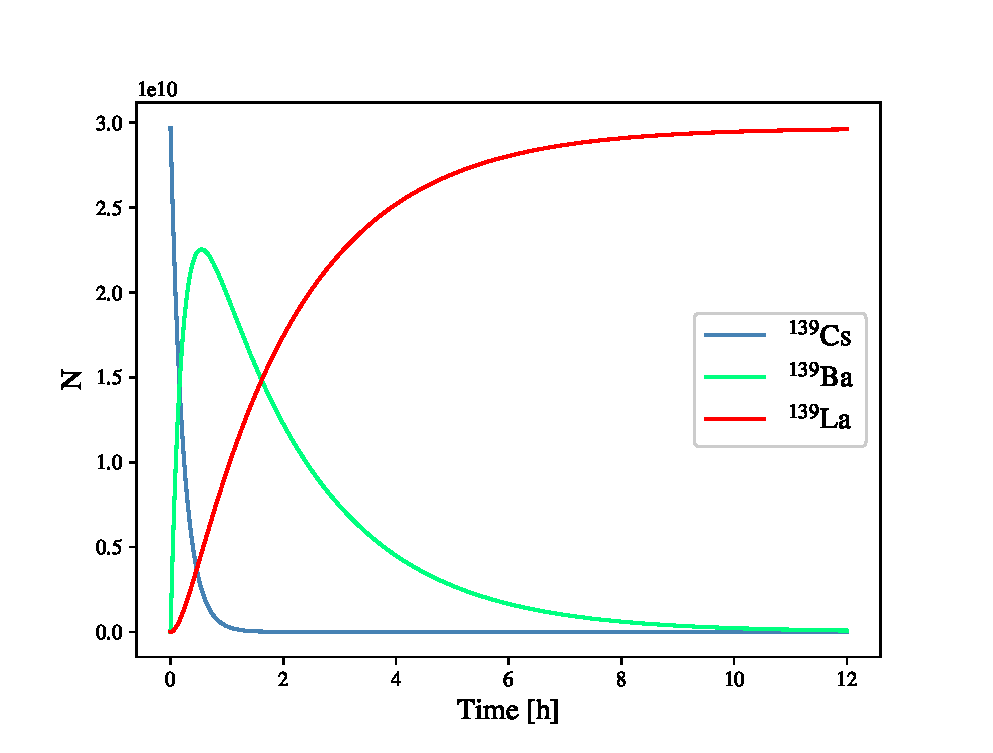
\includegraphics[scale=0.8]{ex7/decay.eps}
    \caption{Number of atoms as a function of time in the decay chain}
    \label{fig:decay_chain}
\end{figure}

\begin{figure}[htbp]
    \centering
    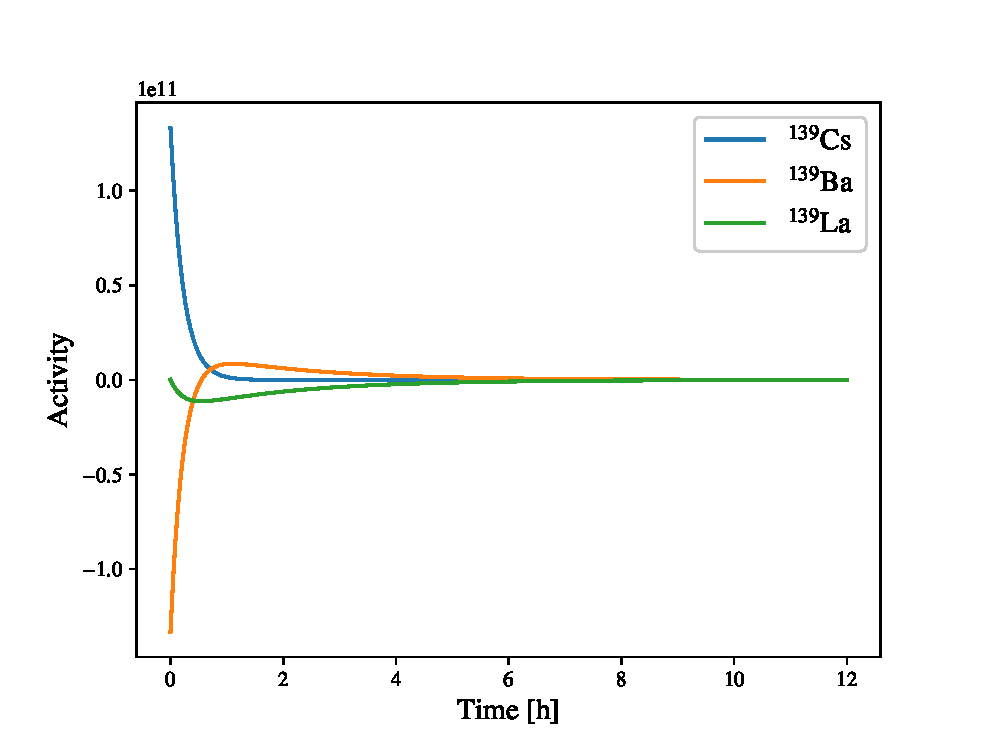
\includegraphics[scale=0.8]{ex7/decay_activities.eps}
    \caption{Activities as a function of time in the decay chain}
    \label{fig:decay_chain_activities}
\end{figure}

Figures \ref{fig:decay_chain} and \ref{fig:decay_chain_activities} report respectively
the number of atoms and the activities as functions of time. Of course at time $t=0$ the only present nuclei are $^{139}$Cs, and as the time passes 
the number of $^{139}$Cs nuclei decreases, while the two other elements start forming in chain. The activity of the first reaction is proportional to the 
the number of atoms of $^{139}$Cs, hence it is logical that the maximum activity of the first reaction is at the beginning of the simulation. For what concerns
$^{139}$Ba, the activity grows as more $^{139}$Ba atoms are produced but a certain point the rate of production of $^{139}$La overcomes the rate of decay of $^{139}$Cs,
and the $^{139}$Ba activity starts decreasing. Finally, the activity of $^{139}$La is always $0$ because no decays are observed

\subsubsection*{e}
The maximum activity of $^{139}$Ba is registered after $33$ minutes, with a maximum value of $3.1391~MBq = 0.0848~mCi$.

\subsubsection*{f}
The activities of $^{139}$Cs and $^{139}$Ba become equal after $0.33$ minutes (see script below), that is in the peak of the activity of  $^{139}$Ba.

\section{Code for ex2}
\lstinputlisting[language=python, showstringspaces=false]{ex2/ex2.py}

\section{Code for ex3}
\lstinputlisting[language=python, showstringspaces=false]{ex3/higgs.py}

\section{Code for ex7}
\lstinputlisting[language=python, showstringspaces=false]{ex7/ex7.py}

\end{document}